\documentclass[1p]{elsarticle_modified}
%\bibliographystyle{elsarticle-num}

%\usepackage[colorlinks]{hyperref}
%\usepackage{abbrmath_seonhwa} %\Abb, \Ascr, \Acal ,\Abf, \Afrak
\usepackage{amsfonts}
\usepackage{amssymb}
\usepackage{amsmath}
\usepackage{amsthm}
\usepackage{scalefnt}
\usepackage{amsbsy}
\usepackage{kotex}
\usepackage{caption}
\usepackage{subfig}
\usepackage{color}
\usepackage{graphicx}
\usepackage{xcolor} %% white, black, red, green, blue, cyan, magenta, yellow
\usepackage{float}
\usepackage{setspace}
\usepackage{hyperref}

\usepackage{tikz}
\usetikzlibrary{arrows}

\usepackage{multirow}
\usepackage{array} % fixed length table
\usepackage{hhline}

%%%%%%%%%%%%%%%%%%%%%
\makeatletter
\renewcommand*\env@matrix[1][\arraystretch]{%
	\edef\arraystretch{#1}%
	\hskip -\arraycolsep
	\let\@ifnextchar\new@ifnextchar
	\array{*\c@MaxMatrixCols c}}
\makeatother %https://tex.stackexchange.com/questions/14071/how-can-i-increase-the-line-spacing-in-a-matrix
%%%%%%%%%%%%%%%

\usepackage[normalem]{ulem}

\newcommand{\msout}[1]{\ifmmode\text{\sout{\ensuremath{#1}}}\else\sout{#1}\fi}
%SOURCE: \msout is \stkout macro in https://tex.stackexchange.com/questions/20609/strikeout-in-math-mode

\newcommand{\cancel}[1]{
	\ifmmode
	{\color{red}\msout{#1}}
	\else
	{\color{red}\sout{#1}}
	\fi
}

\newcommand{\add}[1]{
	{\color{blue}\uwave{#1}}
}

\newcommand{\replace}[2]{
	\ifmmode
	{\color{red}\msout{#1}}{\color{blue}\uwave{#2}}
	\else
	{\color{red}\sout{#1}}{\color{blue}\uwave{#2}}
	\fi
}

\newcommand{\Sol}{\mathcal{S}} %segment
\newcommand{\D}{D} %diagram
\newcommand{\A}{\mathcal{A}} %arc


%%%%%%%%%%%%%%%%%%%%%%%%%%%%%5 test

\def\sl{\operatorname{\textup{SL}}(2,\Cbb)}
\def\psl{\operatorname{\textup{PSL}}(2,\Cbb)}
\def\quan{\mkern 1mu \triangleright \mkern 1mu}

\theoremstyle{definition}
\newtheorem{thm}{Theorem}[section]
\newtheorem{prop}[thm]{Proposition}
\newtheorem{lem}[thm]{Lemma}
\newtheorem{ques}[thm]{Question}
\newtheorem{cor}[thm]{Corollary}
\newtheorem{defn}[thm]{Definition}
\newtheorem{exam}[thm]{Example}
\newtheorem{rmk}[thm]{Remark}
\newtheorem{alg}[thm]{Algorithm}

\newcommand{\I}{\sqrt{-1}}
\begin{document}

%\begin{frontmatter}
%
%\title{Boundary parabolic representations of knots up to 8 crossings}
%
%%% Group authors per affiliation:
%\author{Yunhi Cho} 
%\address{Department of Mathematics, University of Seoul, Seoul, Korea}
%\ead{yhcho@uos.ac.kr}
%
%
%\author{Seonhwa Kim} %\fnref{s_kim}}
%\address{Center for Geometry and Physics, Institute for Basic Science, Pohang, 37673, Korea}
%\ead{ryeona17@ibs.re.kr}
%
%\author{Hyuk Kim}
%\address{Department of Mathematical Sciences, Seoul National University, Seoul 08826, Korea}
%\ead{hyukkim@snu.ac.kr}
%
%\author{Seokbeom Yoon}
%\address{Department of Mathematical Sciences, Seoul National University, Seoul, 08826,  Korea}
%\ead{sbyoon15@snu.ac.kr}
%
%\begin{abstract}
%We find all boundary parabolic representation of knots up to 8 crossings.
%
%\end{abstract}
%\begin{keyword}
%    \MSC[2010] 57M25 
%\end{keyword}
%
%\end{frontmatter}

%\linenumbers
%\tableofcontents
%
\newcommand\colored[1]{\textcolor{white}{\rule[-0.35ex]{0.8em}{1.4ex}}\kern-0.8em\color{red} #1}%
%\newcommand\colored[1]{\textcolor{white}{ #1}\kern-2.17ex	\textcolor{white}{ #1}\kern-1.81ex	\textcolor{white}{ #1}\kern-2.15ex\color{red}#1	}

{\Large $\underline{12n_{0557}~(K12n_{0557})}$}

\setlength{\tabcolsep}{10pt}
\renewcommand{\arraystretch}{1.6}
\vspace{1cm}\begin{tabular}{m{100pt}>{\centering\arraybackslash}m{274pt}}
\multirow{5}{120pt}{
	\centering
	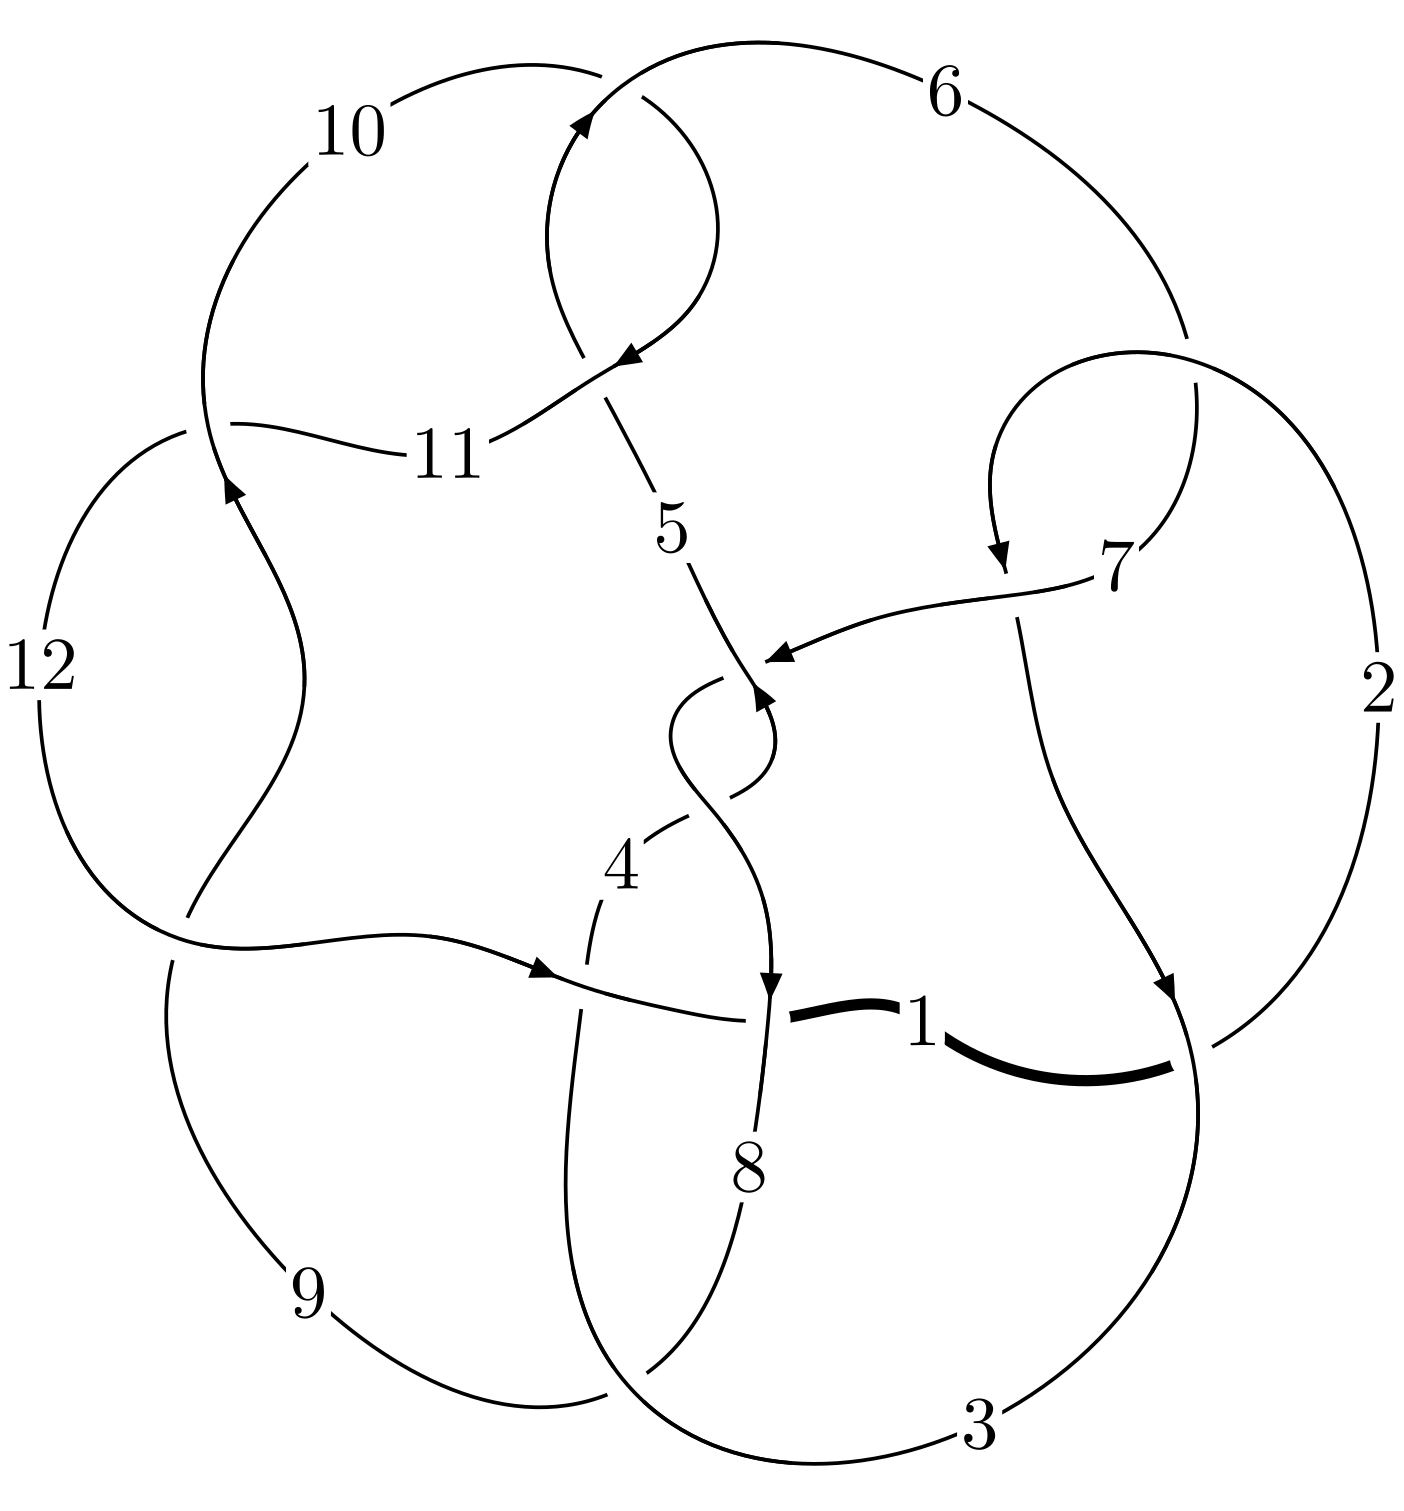
\includegraphics[width=112pt]{../../../GIT/diagram.site/Diagrams/png/2646_12n_0557.png}\\
\ \ \ A knot diagram\footnotemark}&
\allowdisplaybreaks
\textbf{Linearized knot diagam} \\
\cline{2-2}
 &
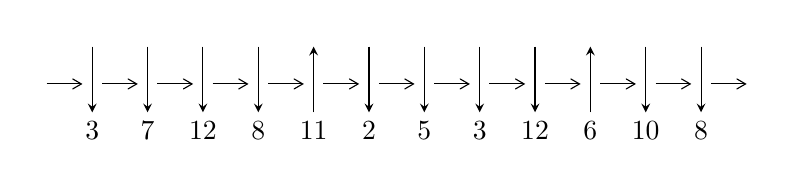
\begin{tikzpicture}[x=20pt, y=17pt]
	% nodes
	\node (C0) at (0, 0) {};
	\node (C1) at (1, 0) {};
	\node (C1U) at (1, +1) {};
	\node (C1D) at (1, -1) {3};

	\node (C2) at (2, 0) {};
	\node (C2U) at (2, +1) {};
	\node (C2D) at (2, -1) {7};

	\node (C3) at (3, 0) {};
	\node (C3U) at (3, +1) {};
	\node (C3D) at (3, -1) {12};

	\node (C4) at (4, 0) {};
	\node (C4U) at (4, +1) {};
	\node (C4D) at (4, -1) {8};

	\node (C5) at (5, 0) {};
	\node (C5U) at (5, +1) {};
	\node (C5D) at (5, -1) {11};

	\node (C6) at (6, 0) {};
	\node (C6U) at (6, +1) {};
	\node (C6D) at (6, -1) {2};

	\node (C7) at (7, 0) {};
	\node (C7U) at (7, +1) {};
	\node (C7D) at (7, -1) {5};

	\node (C8) at (8, 0) {};
	\node (C8U) at (8, +1) {};
	\node (C8D) at (8, -1) {3};

	\node (C9) at (9, 0) {};
	\node (C9U) at (9, +1) {};
	\node (C9D) at (9, -1) {12};

	\node (C10) at (10, 0) {};
	\node (C10U) at (10, +1) {};
	\node (C10D) at (10, -1) {6};

	\node (C11) at (11, 0) {};
	\node (C11U) at (11, +1) {};
	\node (C11D) at (11, -1) {10};

	\node (C12) at (12, 0) {};
	\node (C12U) at (12, +1) {};
	\node (C12D) at (12, -1) {8};
	\node (C13) at (13, 0) {};

	% arrows
	\draw[->,>={angle 60}]
	(C0) edge (C1) (C1) edge (C2) (C2) edge (C3) (C3) edge (C4) (C4) edge (C5) (C5) edge (C6) (C6) edge (C7) (C7) edge (C8) (C8) edge (C9) (C9) edge (C10) (C10) edge (C11) (C11) edge (C12) (C12) edge (C13) ;	\draw[->,>=stealth]
	(C1U) edge (C1D) (C2U) edge (C2D) (C3U) edge (C3D) (C4U) edge (C4D) (C5D) edge (C5U) (C6U) edge (C6D) (C7U) edge (C7D) (C8U) edge (C8D) (C9U) edge (C9D) (C10D) edge (C10U) (C11U) edge (C11D) (C12U) edge (C12D) ;
	\end{tikzpicture} \\
\hhline{~~} \\& 
\textbf{Solving Sequence} \\ \cline{2-2} 
 &
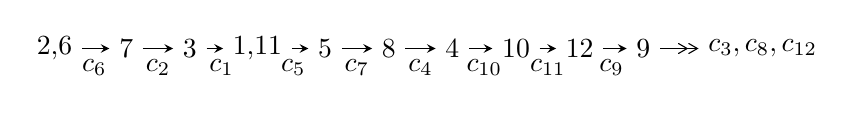
\begin{tikzpicture}[x=23pt, y=7pt]
	% node
	\node (A0) at (-1/8, 0) {2,6};
	\node (A1) at (1, 0) {7};
	\node (A2) at (2, 0) {3};
	\node (A3) at (49/16, 0) {1,11};
	\node (A4) at (33/8, 0) {5};
	\node (A5) at (41/8, 0) {8};
	\node (A6) at (49/8, 0) {4};
	\node (A7) at (57/8, 0) {10};
	\node (A8) at (65/8, 0) {12};
	\node (A9) at (73/8, 0) {9};
	\node (C1) at (1/2, -1) {$c_{6}$};
	\node (C2) at (3/2, -1) {$c_{2}$};
	\node (C3) at (5/2, -1) {$c_{1}$};
	\node (C4) at (29/8, -1) {$c_{5}$};
	\node (C5) at (37/8, -1) {$c_{7}$};
	\node (C6) at (45/8, -1) {$c_{4}$};
	\node (C7) at (53/8, -1) {$c_{10}$};
	\node (C8) at (61/8, -1) {$c_{11}$};
	\node (C9) at (69/8, -1) {$c_{9}$};
	\node (A10) at (11, 0) {$c_{3},c_{8},c_{12}$};

	% edge
	\draw[->,>=stealth]	
	(A0) edge (A1) (A1) edge (A2) (A2) edge (A3) (A3) edge (A4) (A4) edge (A5) (A5) edge (A6) (A6) edge (A7) (A7) edge (A8) (A8) edge (A9) ;
	\draw[->>,>={angle 60}]	
	(A9) edge (A10);
\end{tikzpicture} \\ 

\end{tabular} \\

\footnotetext{
The image of knot diagram is generated by the software ``\textbf{Draw programme}" developed by Andrew Bartholomew(\url{http://www.layer8.co.uk/maths/draw/index.htm\#Running-draw}), where we modified some parts for our purpose(\url{https://github.com/CATsTAILs/LinksPainter}).
}\phantom \\ \newline 
\centering \textbf{Ideals for irreducible components\footnotemark of $X_{\text{par}}$} 
 
\begin{align*}
I^u_{1}&=\langle 
-1.02105\times10^{101} u^{67}-4.63803\times10^{101} u^{66}+\cdots+1.96878\times10^{102} b-8.88022\times10^{101},\\
\phantom{I^u_{1}}&\phantom{= \langle  }1.26302\times10^{102} u^{67}+8.85176\times10^{101} u^{66}+\cdots+1.96878\times10^{102} a+1.15700\times10^{102},\;u^{68}+u^{67}+\cdots+u-1\rangle \\
I^u_{2}&=\langle 
-5 u^{19}+33 u^{17}+\cdots+b+11 u,\;-11 u^{18}-2 u^{17}+\cdots+a+29,\;u^{20}-7 u^{18}+\cdots+u+1\rangle \\
\\
\end{align*}
\raggedright * 2 irreducible components of $\dim_{\mathbb{C}}=0$, with total 88 representations.\\
\footnotetext{All coefficients of polynomials are rational numbers. But the coefficients are sometimes approximated in decimal forms when there is not enough margin.}
\newpage
\renewcommand{\arraystretch}{1}
\centering \section*{I. $I^u_{1}= \langle -1.02\times10^{101} u^{67}-4.64\times10^{101} u^{66}+\cdots+1.97\times10^{102} b-8.88\times10^{101},\;1.26\times10^{102} u^{67}+8.85\times10^{101} u^{66}+\cdots+1.97\times10^{102} a+1.16\times10^{102},\;u^{68}+u^{67}+\cdots+u-1 \rangle$}
\flushleft \textbf{(i) Arc colorings}\\
\begin{tabular}{m{7pt} m{180pt} m{7pt} m{180pt} }
\flushright $a_{2}=$&$\begin{pmatrix}0\\u\end{pmatrix}$ \\
\flushright $a_{6}=$&$\begin{pmatrix}1\\0\end{pmatrix}$ \\
\flushright $a_{7}=$&$\begin{pmatrix}1\\u^2\end{pmatrix}$ \\
\flushright $a_{3}=$&$\begin{pmatrix}- u\\- u^3+u\end{pmatrix}$ \\
\flushright $a_{1}=$&$\begin{pmatrix}u^3\\u^5- u^3+u\end{pmatrix}$ \\
\flushright $a_{11}=$&$\begin{pmatrix}-0.641523 u^{67}-0.449607 u^{66}+\cdots+0.395110 u-0.587676\\0.0518621 u^{67}+0.235579 u^{66}+\cdots-1.81551 u+0.451053\end{pmatrix}$ \\
\flushright $a_{5}=$&$\begin{pmatrix}-0.458253 u^{67}-0.528500 u^{66}+\cdots+2.40287 u-0.615703\\0.243980 u^{67}+0.462555 u^{66}+\cdots-2.28263 u-0.185736\end{pmatrix}$ \\
\flushright $a_{8}=$&$\begin{pmatrix}0.141644 u^{67}-0.134104 u^{66}+\cdots-1.04997 u+2.16525\\-0.308718 u^{67}-0.377649 u^{66}+\cdots+1.18451 u-1.47282\end{pmatrix}$ \\
\flushright $a_{4}=$&$\begin{pmatrix}0.736347 u^{67}+0.739432 u^{66}+\cdots+0.595559 u-0.749166\\-0.210641 u^{67}-0.118772 u^{66}+\cdots+0.845338 u+0.371913\end{pmatrix}$ \\
\flushright $a_{10}=$&$\begin{pmatrix}-0.693385 u^{67}-0.685186 u^{66}+\cdots+2.21062 u-1.03873\\0.0518621 u^{67}+0.235579 u^{66}+\cdots-1.81551 u+0.451053\end{pmatrix}$ \\
\flushright $a_{12}=$&$\begin{pmatrix}-0.704846 u^{67}-1.06386 u^{66}+\cdots+4.02275 u-0.154197\\0.263760 u^{67}+0.386209 u^{66}+\cdots-1.73388 u-0.866876\end{pmatrix}$ \\
\flushright $a_{9}=$&$\begin{pmatrix}0.147546 u^{67}-0.0835648 u^{66}+\cdots-1.04362 u+2.37990\\-0.325349 u^{67}-0.435020 u^{66}+\cdots+1.13942 u-1.64284\end{pmatrix}$\\&\end{tabular}
\flushleft \textbf{(ii) Obstruction class $= -1$}\\~\\
\flushleft \textbf{(iii) Cusp Shapes $= -0.626539 u^{67}-1.34740 u^{66}+\cdots+9.36366 u-10.4358$}\\~\\
\newpage\renewcommand{\arraystretch}{1}
\flushleft \textbf{(iv) u-Polynomials at the component}\newline \\
\begin{tabular}{m{50pt}|m{274pt}}
Crossings & \hspace{64pt}u-Polynomials at each crossing \\
\hline $$\begin{aligned}c_{1}\end{aligned}$$&$\begin{aligned}
&u^{68}+37 u^{67}+\cdots- u+1
\end{aligned}$\\
\hline $$\begin{aligned}c_{2},c_{6}\end{aligned}$$&$\begin{aligned}
&u^{68}- u^{67}+\cdots- u-1
\end{aligned}$\\
\hline $$\begin{aligned}c_{3}\end{aligned}$$&$\begin{aligned}
&u^{68}-3 u^{67}+\cdots-5590 u-1393
\end{aligned}$\\
\hline $$\begin{aligned}c_{4},c_{7}\end{aligned}$$&$\begin{aligned}
&u^{68}-2 u^{67}+\cdots+682 u+107
\end{aligned}$\\
\hline $$\begin{aligned}c_{5},c_{10}\end{aligned}$$&$\begin{aligned}
&u^{68}+u^{67}+\cdots-5 u+1
\end{aligned}$\\
\hline $$\begin{aligned}c_{8}\end{aligned}$$&$\begin{aligned}
&u^{68}+u^{67}+\cdots-2029 u-1341
\end{aligned}$\\
\hline $$\begin{aligned}c_{9},c_{11}\end{aligned}$$&$\begin{aligned}
&u^{68}+25 u^{67}+\cdots-57 u+1
\end{aligned}$\\
\hline $$\begin{aligned}c_{12}\end{aligned}$$&$\begin{aligned}
&u^{68}-3 u^{67}+\cdots+2287 u+121
\end{aligned}$\\
\hline
\end{tabular}\\~\\
\newpage\renewcommand{\arraystretch}{1}
\flushleft \textbf{(v) Riley Polynomials at the component}\newline \\
\begin{tabular}{m{50pt}|m{274pt}}
Crossings & \hspace{64pt}Riley Polynomials at each crossing \\
\hline $$\begin{aligned}c_{1}\end{aligned}$$&$\begin{aligned}
&y^{68}+3 y^{67}+\cdots+105 y+1
\end{aligned}$\\
\hline $$\begin{aligned}c_{2},c_{6}\end{aligned}$$&$\begin{aligned}
&y^{68}-37 y^{67}+\cdots+y+1
\end{aligned}$\\
\hline $$\begin{aligned}c_{3}\end{aligned}$$&$\begin{aligned}
&y^{68}-69 y^{67}+\cdots-13063878 y+1940449
\end{aligned}$\\
\hline $$\begin{aligned}c_{4},c_{7}\end{aligned}$$&$\begin{aligned}
&y^{68}+28 y^{67}+\cdots-23856 y+11449
\end{aligned}$\\
\hline $$\begin{aligned}c_{5},c_{10}\end{aligned}$$&$\begin{aligned}
&y^{68}+25 y^{67}+\cdots-57 y+1
\end{aligned}$\\
\hline $$\begin{aligned}c_{8}\end{aligned}$$&$\begin{aligned}
&y^{68}-67 y^{67}+\cdots+17462531 y+1798281
\end{aligned}$\\
\hline $$\begin{aligned}c_{9},c_{11}\end{aligned}$$&$\begin{aligned}
&y^{68}+45 y^{67}+\cdots-977 y+1
\end{aligned}$\\
\hline $$\begin{aligned}c_{12}\end{aligned}$$&$\begin{aligned}
&y^{68}-75 y^{67}+\cdots-4777829 y+14641
\end{aligned}$\\
\hline
\end{tabular}\\~\\
\newpage\flushleft \textbf{(vi) Complex Volumes and Cusp Shapes}
$$\begin{array}{c|c|c}  
\text{Solutions to }I^u_{1}& \I (\text{vol} + \sqrt{-1}CS) & \text{Cusp shape}\\
 \hline 
\begin{aligned}
u &= \phantom{-}0.940907 + 0.259610 I \\
a &= \phantom{-}0.42197 - 2.48976 I \\
b &= -0.159587 - 1.033910 I\end{aligned}
 & -0.93999 - 1.07351 I & -13.16109 - 0.94732 I \\ \hline\begin{aligned}
u &= \phantom{-}0.940907 - 0.259610 I \\
a &= \phantom{-}0.42197 + 2.48976 I \\
b &= -0.159587 + 1.033910 I\end{aligned}
 & -0.93999 + 1.07351 I & -13.16109 + 0.94732 I \\ \hline\begin{aligned}
u &= -1.043650 + 0.145685 I \\
a &= -0.39955 + 2.55386 I \\
b &= \phantom{-}0.275203 + 0.962008 I\end{aligned}
 & -3.76897 + 2.72988 I & -8.00000 - 5.48520 I \\ \hline\begin{aligned}
u &= -1.043650 - 0.145685 I \\
a &= -0.39955 - 2.55386 I \\
b &= \phantom{-}0.275203 - 0.962008 I\end{aligned}
 & -3.76897 - 2.72988 I & -8.00000 + 5.48520 I \\ \hline\begin{aligned}
u &= \phantom{-}0.885464 + 0.597578 I \\
a &= \phantom{-}0.75942 + 1.75588 I \\
b &= \phantom{-}0.093114 + 0.992704 I\end{aligned}
 & -1.11071 - 2.33001 I & \phantom{-0.000000 } 0 \\ \hline\begin{aligned}
u &= \phantom{-}0.885464 - 0.597578 I \\
a &= \phantom{-}0.75942 - 1.75588 I \\
b &= \phantom{-}0.093114 - 0.992704 I\end{aligned}
 & -1.11071 + 2.33001 I & \phantom{-0.000000 } 0 \\ \hline\begin{aligned}
u &= -1.004080 + 0.415754 I \\
a &= \phantom{-}0.232891 - 0.695090 I \\
b &= -0.812580 + 0.667456 I\end{aligned}
 & -4.35054 + 1.56377 I & \phantom{-0.000000 } 0 \\ \hline\begin{aligned}
u &= -1.004080 - 0.415754 I \\
a &= \phantom{-}0.232891 + 0.695090 I \\
b &= -0.812580 - 0.667456 I\end{aligned}
 & -4.35054 - 1.56377 I & \phantom{-0.000000 } 0 \\ \hline\begin{aligned}
u &= -0.876146 + 0.645556 I \\
a &= \phantom{-}0.163390 + 0.383509 I \\
b &= -0.159247 - 0.049954 I\end{aligned}
 & \phantom{-}2.13037 + 2.54033 I & \phantom{-0.000000 } 0 \\ \hline\begin{aligned}
u &= -0.876146 - 0.645556 I \\
a &= \phantom{-}0.163390 - 0.383509 I \\
b &= -0.159247 + 0.049954 I\end{aligned}
 & \phantom{-}2.13037 - 2.54033 I & \phantom{-0.000000 } 0\\
 \hline 
 \end{array}$$\newpage$$\begin{array}{c|c|c}  
\text{Solutions to }I^u_{1}& \I (\text{vol} + \sqrt{-1}CS) & \text{Cusp shape}\\
 \hline 
\begin{aligned}
u &= \phantom{-}0.399517 + 1.015870 I \\
a &= \phantom{-}0.654911 + 0.379579 I \\
b &= -0.849945 + 0.659975 I\end{aligned}
 & \phantom{-}0.65883 + 3.48006 I & \phantom{-0.000000 } 0 \\ \hline\begin{aligned}
u &= \phantom{-}0.399517 - 1.015870 I \\
a &= \phantom{-}0.654911 - 0.379579 I \\
b &= -0.849945 - 0.659975 I\end{aligned}
 & \phantom{-}0.65883 - 3.48006 I & \phantom{-0.000000 } 0 \\ \hline\begin{aligned}
u &= -1.037540 + 0.398544 I \\
a &= -0.14880 + 1.55501 I \\
b &= -0.576579 + 1.193350 I\end{aligned}
 & -6.36651 - 0.81288 I & \phantom{-0.000000 } 0 \\ \hline\begin{aligned}
u &= -1.037540 - 0.398544 I \\
a &= -0.14880 - 1.55501 I \\
b &= -0.576579 - 1.193350 I\end{aligned}
 & -6.36651 + 0.81288 I & \phantom{-0.000000 } 0 \\ \hline\begin{aligned}
u &= \phantom{-}0.716409 + 0.891799 I \\
a &= \phantom{-}0.500992 - 0.440317 I \\
b &= -0.674233 - 0.922387 I\end{aligned}
 & \phantom{-}3.29939 + 2.00709 I & \phantom{-0.000000 } 0 \\ \hline\begin{aligned}
u &= \phantom{-}0.716409 - 0.891799 I \\
a &= \phantom{-}0.500992 + 0.440317 I \\
b &= -0.674233 + 0.922387 I\end{aligned}
 & \phantom{-}3.29939 - 2.00709 I & \phantom{-0.000000 } 0 \\ \hline\begin{aligned}
u &= -0.342929 + 1.097870 I \\
a &= \phantom{-}0.556771 + 0.538161 I \\
b &= -0.723860 + 1.040460 I\end{aligned}
 & -0.50810 - 9.35376 I & \phantom{-0.000000 } 0 \\ \hline\begin{aligned}
u &= -0.342929 - 1.097870 I \\
a &= \phantom{-}0.556771 - 0.538161 I \\
b &= -0.723860 - 1.040460 I\end{aligned}
 & -0.50810 + 9.35376 I & \phantom{-0.000000 } 0 \\ \hline\begin{aligned}
u &= -0.098391 + 0.835496 I \\
a &= \phantom{-}0.643296 - 0.760427 I \\
b &= \phantom{-}0.141512 - 1.090530 I\end{aligned}
 & -6.10032 - 3.11040 I & -10.83046 + 2.94729 I \\ \hline\begin{aligned}
u &= -0.098391 - 0.835496 I \\
a &= \phantom{-}0.643296 + 0.760427 I \\
b &= \phantom{-}0.141512 + 1.090530 I\end{aligned}
 & -6.10032 + 3.11040 I & -10.83046 - 2.94729 I\\
 \hline 
 \end{array}$$\newpage$$\begin{array}{c|c|c}  
\text{Solutions to }I^u_{1}& \I (\text{vol} + \sqrt{-1}CS) & \text{Cusp shape}\\
 \hline 
\begin{aligned}
u &= \phantom{-}1.046410 + 0.508419 I \\
a &= -0.132346 + 0.527696 I \\
b &= -0.940830 + 0.317450 I\end{aligned}
 & -3.60038 - 4.71726 I & \phantom{-0.000000 } 0 \\ \hline\begin{aligned}
u &= \phantom{-}1.046410 - 0.508419 I \\
a &= -0.132346 - 0.527696 I \\
b &= -0.940830 - 0.317450 I\end{aligned}
 & -3.60038 + 4.71726 I & \phantom{-0.000000 } 0 \\ \hline\begin{aligned}
u &= -0.768060 + 0.318425 I \\
a &= -2.70476 + 2.59441 I \\
b &= \phantom{-}0.549168 + 0.792945 I\end{aligned}
 & -3.34454 + 1.57597 I & -9.61436 - 5.33785 I \\ \hline\begin{aligned}
u &= -0.768060 - 0.318425 I \\
a &= -2.70476 - 2.59441 I \\
b &= \phantom{-}0.549168 - 0.792945 I\end{aligned}
 & -3.34454 - 1.57597 I & -9.61436 + 5.33785 I \\ \hline\begin{aligned}
u &= \phantom{-}1.047410 + 0.527364 I \\
a &= \phantom{-}1.61700 + 1.10646 I \\
b &= -0.706839 + 1.027240 I\end{aligned}
 & -5.45556 - 7.28309 I & \phantom{-0.000000 } 0 \\ \hline\begin{aligned}
u &= \phantom{-}1.047410 - 0.527364 I \\
a &= \phantom{-}1.61700 - 1.10646 I \\
b &= -0.706839 - 1.027240 I\end{aligned}
 & -5.45556 + 7.28309 I & \phantom{-0.000000 } 0 \\ \hline\begin{aligned}
u &= \phantom{-}1.083690 + 0.530024 I \\
a &= -0.553710 - 0.091586 I \\
b &= -0.851770 - 0.802509 I\end{aligned}
 & \phantom{-}3.49437 - 0.97425 I & \phantom{-0.000000 } 0 \\ \hline\begin{aligned}
u &= \phantom{-}1.083690 - 0.530024 I \\
a &= -0.553710 + 0.091586 I \\
b &= -0.851770 + 0.802509 I\end{aligned}
 & \phantom{-}3.49437 + 0.97425 I & \phantom{-0.000000 } 0 \\ \hline\begin{aligned}
u &= -0.934372 + 0.781624 I \\
a &= \phantom{-}0.053522 + 0.417489 I \\
b &= \phantom{-}0.680894 - 0.644957 I\end{aligned}
 & \phantom{-}3.42338 + 2.92327 I & \phantom{-0.000000 } 0 \\ \hline\begin{aligned}
u &= -0.934372 - 0.781624 I \\
a &= \phantom{-}0.053522 - 0.417489 I \\
b &= \phantom{-}0.680894 + 0.644957 I\end{aligned}
 & \phantom{-}3.42338 - 2.92327 I & \phantom{-0.000000 } 0\\
 \hline 
 \end{array}$$\newpage$$\begin{array}{c|c|c}  
\text{Solutions to }I^u_{1}& \I (\text{vol} + \sqrt{-1}CS) & \text{Cusp shape}\\
 \hline 
\begin{aligned}
u &= -0.841651 + 0.883672 I \\
a &= \phantom{-}0.868517 - 0.485589 I \\
b &= -0.677512 - 0.774206 I\end{aligned}
 & \phantom{-}3.75199 + 3.22331 I & \phantom{-0.000000 } 0 \\ \hline\begin{aligned}
u &= -0.841651 - 0.883672 I \\
a &= \phantom{-}0.868517 + 0.485589 I \\
b &= -0.677512 + 0.774206 I\end{aligned}
 & \phantom{-}3.75199 - 3.22331 I & \phantom{-0.000000 } 0 \\ \hline\begin{aligned}
u &= \phantom{-}0.548357 + 0.532260 I \\
a &= -0.28832 - 1.56425 I \\
b &= \phantom{-}0.576815 + 0.947312 I\end{aligned}
 & -3.88368 + 2.91929 I & -8.58150 - 1.60014 I \\ \hline\begin{aligned}
u &= \phantom{-}0.548357 - 0.532260 I \\
a &= -0.28832 + 1.56425 I \\
b &= \phantom{-}0.576815 - 0.947312 I\end{aligned}
 & -3.88368 - 2.91929 I & -8.58150 + 1.60014 I \\ \hline\begin{aligned}
u &= -1.24899\phantom{ +0.000000I} \\
a &= -1.01889\phantom{ +0.000000I} \\
b &= \phantom{-}0.341297\phantom{ +0.000000I}\end{aligned}
 & -6.77611\phantom{ +0.000000I} & \phantom{-0.000000 } 0 \\ \hline\begin{aligned}
u &= \phantom{-}0.750601\phantom{ +0.000000I} \\
a &= \phantom{-}0.454925\phantom{ +0.000000I} \\
b &= \phantom{-}0.481221\phantom{ +0.000000I}\end{aligned}
 & -1.11068\phantom{ +0.000000I} & -8.83830\phantom{ +0.000000I} \\ \hline\begin{aligned}
u &= -1.157710 + 0.488774 I \\
a &= \phantom{-}0.89610 - 1.78056 I \\
b &= -0.790649 - 0.975806 I\end{aligned}
 & \phantom{-}2.95487 + 7.09497 I & \phantom{-0.000000 } 0 \\ \hline\begin{aligned}
u &= -1.157710 - 0.488774 I \\
a &= \phantom{-}0.89610 + 1.78056 I \\
b &= -0.790649 + 0.975806 I\end{aligned}
 & \phantom{-}2.95487 - 7.09497 I & \phantom{-0.000000 } 0 \\ \hline\begin{aligned}
u &= \phantom{-}1.019200 + 0.755143 I \\
a &= -1.43617 - 1.55373 I \\
b &= \phantom{-}0.644876 - 1.003110 I\end{aligned}
 & \phantom{-}2.34696 - 8.08537 I & \phantom{-0.000000 } 0 \\ \hline\begin{aligned}
u &= \phantom{-}1.019200 - 0.755143 I \\
a &= -1.43617 + 1.55373 I \\
b &= \phantom{-}0.644876 + 1.003110 I\end{aligned}
 & \phantom{-}2.34696 + 8.08537 I & \phantom{-0.000000 } 0\\
 \hline 
 \end{array}$$\newpage$$\begin{array}{c|c|c}  
\text{Solutions to }I^u_{1}& \I (\text{vol} + \sqrt{-1}CS) & \text{Cusp shape}\\
 \hline 
\begin{aligned}
u &= -1.137780 + 0.597361 I \\
a &= -0.680702 + 0.371018 I \\
b &= -0.611829 + 0.671402 I\end{aligned}
 & \phantom{-}2.91478 + 2.04568 I & \phantom{-0.000000 } 0 \\ \hline\begin{aligned}
u &= -1.137780 - 0.597361 I \\
a &= -0.680702 - 0.371018 I \\
b &= -0.611829 - 0.671402 I\end{aligned}
 & \phantom{-}2.91478 - 2.04568 I & \phantom{-0.000000 } 0 \\ \hline\begin{aligned}
u &= \phantom{-}1.210900 + 0.474728 I \\
a &= \phantom{-}0.58877 + 2.13386 I \\
b &= -0.619959 + 0.991046 I\end{aligned}
 & \phantom{-}1.92170 - 6.94863 I & \phantom{-0.000000 } 0 \\ \hline\begin{aligned}
u &= \phantom{-}1.210900 - 0.474728 I \\
a &= \phantom{-}0.58877 - 2.13386 I \\
b &= -0.619959 - 0.991046 I\end{aligned}
 & \phantom{-}1.92170 + 6.94863 I & \phantom{-0.000000 } 0 \\ \hline\begin{aligned}
u &= -1.188350 + 0.530219 I \\
a &= \phantom{-}0.57443 - 1.99425 I \\
b &= -0.133485 - 1.246610 I\end{aligned}
 & -9.23070 + 8.01469 I & \phantom{-0.000000 } 0 \\ \hline\begin{aligned}
u &= -1.188350 - 0.530219 I \\
a &= \phantom{-}0.57443 + 1.99425 I \\
b &= -0.133485 + 1.246610 I\end{aligned}
 & -9.23070 - 8.01469 I & \phantom{-0.000000 } 0 \\ \hline\begin{aligned}
u &= \phantom{-}0.444105 + 0.517971 I \\
a &= \phantom{-}0.608976 - 0.934274 I \\
b &= \phantom{-}0.732751 + 0.181612 I\end{aligned}
 & -1.85955 + 0.48121 I & -4.42539 + 0.48875 I \\ \hline\begin{aligned}
u &= \phantom{-}0.444105 - 0.517971 I \\
a &= \phantom{-}0.608976 + 0.934274 I \\
b &= \phantom{-}0.732751 - 0.181612 I\end{aligned}
 & -1.85955 - 0.48121 I & -4.42539 - 0.48875 I \\ \hline\begin{aligned}
u &= -0.172980 + 0.644207 I \\
a &= -0.086216 + 0.618638 I \\
b &= \phantom{-}0.742213 + 0.849423 I\end{aligned}
 & \phantom{-}5.46513 + 2.81095 I & -4.67462 - 2.60873 I \\ \hline\begin{aligned}
u &= -0.172980 - 0.644207 I \\
a &= -0.086216 - 0.618638 I \\
b &= \phantom{-}0.742213 - 0.849423 I\end{aligned}
 & \phantom{-}5.46513 - 2.81095 I & -4.67462 + 2.60873 I\\
 \hline 
 \end{array}$$\newpage$$\begin{array}{c|c|c}  
\text{Solutions to }I^u_{1}& \I (\text{vol} + \sqrt{-1}CS) & \text{Cusp shape}\\
 \hline 
\begin{aligned}
u &= \phantom{-}1.312170 + 0.378943 I \\
a &= -0.96232 - 1.62440 I \\
b &= \phantom{-}0.069729 - 1.052040 I\end{aligned}
 & -10.44160 - 1.32359 I & \phantom{-0.000000 } 0 \\ \hline\begin{aligned}
u &= \phantom{-}1.312170 - 0.378943 I \\
a &= -0.96232 + 1.62440 I \\
b &= \phantom{-}0.069729 + 1.052040 I\end{aligned}
 & -10.44160 + 1.32359 I & \phantom{-0.000000 } 0 \\ \hline\begin{aligned}
u &= -0.587051 + 0.229586 I \\
a &= -0.76768 + 3.66509 I \\
b &= \phantom{-}0.455736 + 1.134590 I\end{aligned}
 & -4.71625 + 3.83876 I & -6.01425 - 8.08352 I \\ \hline\begin{aligned}
u &= -0.587051 - 0.229586 I \\
a &= -0.76768 - 3.66509 I \\
b &= \phantom{-}0.455736 - 1.134590 I\end{aligned}
 & -4.71625 - 3.83876 I & -6.01425 + 8.08352 I \\ \hline\begin{aligned}
u &= \phantom{-}1.192260 + 0.675113 I \\
a &= \phantom{-}0.403435 - 0.199397 I \\
b &= \phantom{-}0.934236 + 0.605763 I\end{aligned}
 & -1.79071 - 9.57598 I & \phantom{-0.000000 } 0 \\ \hline\begin{aligned}
u &= \phantom{-}1.192260 - 0.675113 I \\
a &= \phantom{-}0.403435 + 0.199397 I \\
b &= \phantom{-}0.934236 - 0.605763 I\end{aligned}
 & -1.79071 + 9.57598 I & \phantom{-0.000000 } 0 \\ \hline\begin{aligned}
u &= -1.24627 + 0.68565 I \\
a &= -1.04436 + 1.71892 I \\
b &= \phantom{-}0.735262 + 1.096550 I\end{aligned}
 & -3.3132 + 15.7131 I & \phantom{-0.000000 } 0 \\ \hline\begin{aligned}
u &= -1.24627 - 0.68565 I \\
a &= -1.04436 - 1.71892 I \\
b &= \phantom{-}0.735262 - 1.096550 I\end{aligned}
 & -3.3132 - 15.7131 I & \phantom{-0.000000 } 0 \\ \hline\begin{aligned}
u &= -1.49863 + 0.14703 I \\
a &= -0.238266 + 1.256530 I \\
b &= \phantom{-}0.643640 + 0.677255 I\end{aligned}
 & -6.04640 + 0.52618 I & \phantom{-0.000000 } 0 \\ \hline\begin{aligned}
u &= -1.49863 - 0.14703 I \\
a &= -0.238266 - 1.256530 I \\
b &= \phantom{-}0.643640 - 0.677255 I\end{aligned}
 & -6.04640 - 0.52618 I & \phantom{-0.000000 } 0\\
 \hline 
 \end{array}$$\newpage$$\begin{array}{c|c|c}  
\text{Solutions to }I^u_{1}& \I (\text{vol} + \sqrt{-1}CS) & \text{Cusp shape}\\
 \hline 
\begin{aligned}
u &= \phantom{-}1.52986 + 0.24219 I \\
a &= \phantom{-}0.175494 + 1.248290 I \\
b &= \phantom{-}0.639173 + 0.989620 I\end{aligned}
 & -7.00901 + 4.52551 I & \phantom{-0.000000 } 0 \\ \hline\begin{aligned}
u &= \phantom{-}1.52986 - 0.24219 I \\
a &= \phantom{-}0.175494 - 1.248290 I \\
b &= \phantom{-}0.639173 - 0.989620 I\end{aligned}
 & -7.00901 - 4.52551 I & \phantom{-0.000000 } 0 \\ \hline\begin{aligned}
u &= \phantom{-}0.337839 + 0.292985 I \\
a &= -1.63156 - 0.79539 I \\
b &= \phantom{-}0.841620 - 0.916425 I\end{aligned}
 & \phantom{-}5.70133 - 3.16227 I & -8.17605 + 1.97963 I \\ \hline\begin{aligned}
u &= \phantom{-}0.337839 - 0.292985 I \\
a &= -1.63156 + 0.79539 I \\
b &= \phantom{-}0.841620 + 0.916425 I\end{aligned}
 & \phantom{-}5.70133 + 3.16227 I & -8.17605 - 1.97963 I \\ \hline\begin{aligned}
u &= \phantom{-}0.147872 + 0.344296 I \\
a &= \phantom{-}0.999072 + 0.433594 I \\
b &= -0.214633 + 0.698481 I\end{aligned}
 & -0.427609 - 1.011650 I & -6.71477 + 6.54763 I \\ \hline\begin{aligned}
u &= \phantom{-}0.147872 - 0.344296 I \\
a &= \phantom{-}0.999072 - 0.433594 I \\
b &= -0.214633 - 0.698481 I\end{aligned}
 & -0.427609 + 1.011650 I & -6.71477 - 6.54763 I \\ \hline\begin{aligned}
u &= -0.177594 + 0.322240 I \\
a &= -0.862215 + 0.770131 I \\
b &= \phantom{-}0.836335 - 0.904083 I\end{aligned}
 & \phantom{-}5.73139 - 3.08529 I & -6.85812 + 5.06126 I \\ \hline\begin{aligned}
u &= -0.177594 - 0.322240 I \\
a &= -0.862215 - 0.770131 I \\
b &= \phantom{-}0.836335 + 0.904083 I\end{aligned}
 & \phantom{-}5.73139 + 3.08529 I & -6.85812 - 5.06126 I\\
 \hline 
 \end{array}$$\newpage\newpage\renewcommand{\arraystretch}{1}
\centering \section*{II. $I^u_{2}= \langle -5 u^{19}+33 u^{17}+\cdots+b+11 u,\;-11 u^{18}-2 u^{17}+\cdots+a+29,\;u^{20}-7 u^{18}+\cdots+u+1 \rangle$}
\flushleft \textbf{(i) Arc colorings}\\
\begin{tabular}{m{7pt} m{180pt} m{7pt} m{180pt} }
\flushright $a_{2}=$&$\begin{pmatrix}0\\u\end{pmatrix}$ \\
\flushright $a_{6}=$&$\begin{pmatrix}1\\0\end{pmatrix}$ \\
\flushright $a_{7}=$&$\begin{pmatrix}1\\u^2\end{pmatrix}$ \\
\flushright $a_{3}=$&$\begin{pmatrix}- u\\- u^3+u\end{pmatrix}$ \\
\flushright $a_{1}=$&$\begin{pmatrix}u^3\\u^5- u^3+u\end{pmatrix}$ \\
\flushright $a_{11}=$&$\begin{pmatrix}11 u^{18}+2 u^{17}+\cdots-16 u-29\\5 u^{19}-33 u^{17}+\cdots-11 u^2-11 u\end{pmatrix}$ \\
\flushright $a_{5}=$&$\begin{pmatrix}-3 u^{19}+18 u^{17}+\cdots-3 u+1\\-4 u^{19}+26 u^{17}+\cdots+9 u-1\end{pmatrix}$ \\
\flushright $a_{8}=$&$\begin{pmatrix}- u^{19}+7 u^{17}+\cdots+2 u-6\\u^{19}-2 u^{18}+\cdots-32 u^2+6\end{pmatrix}$ \\
\flushright $a_{4}=$&$\begin{pmatrix}3 u^{19}- u^{18}+\cdots-20 u+8\\-8 u^{19}+u^{18}+\cdots+14 u-6\end{pmatrix}$ \\
\flushright $a_{10}=$&$\begin{pmatrix}-5 u^{19}+11 u^{18}+\cdots-5 u-29\\5 u^{19}-33 u^{17}+\cdots-11 u^2-11 u\end{pmatrix}$ \\
\flushright $a_{12}=$&$\begin{pmatrix}-5 u^{19}+u^{18}+\cdots+17 u-7\\5 u^{19}- u^{18}+\cdots-6 u+5\end{pmatrix}$ \\
\flushright $a_{9}=$&$\begin{pmatrix}- u^{19}+u^{18}+\cdots+u-7\\u^{19}-2 u^{18}+\cdots-33 u^2+6\end{pmatrix}$\\&\end{tabular}
\flushleft \textbf{(ii) Obstruction class $= 1$}\\~\\
\flushleft \textbf{(iii) Cusp Shapes $= -2 u^{19}+4 u^{18}+12 u^{17}-29 u^{16}-32 u^{15}+101 u^{14}+46 u^{13}-224 u^{12}-25 u^{11}+343 u^{10}-29 u^9-382 u^8+73 u^7+319 u^6-76 u^5-197 u^4+45 u^3+92 u^2-18 u-33$}\\~\\
\newpage\renewcommand{\arraystretch}{1}
\flushleft \textbf{(iv) u-Polynomials at the component}\newline \\
\begin{tabular}{m{50pt}|m{274pt}}
Crossings & \hspace{64pt}u-Polynomials at each crossing \\
\hline $$\begin{aligned}c_{1}\end{aligned}$$&$\begin{aligned}
&u^{20}-14 u^{19}+\cdots-15 u+1
\end{aligned}$\\
\hline $$\begin{aligned}c_{2}\end{aligned}$$&$\begin{aligned}
&u^{20}-7 u^{18}+\cdots- u+1
\end{aligned}$\\
\hline $$\begin{aligned}c_{3}\end{aligned}$$&$\begin{aligned}
&u^{20}+6 u^{19}+\cdots+6 u+1
\end{aligned}$\\
\hline $$\begin{aligned}c_{4}\end{aligned}$$&$\begin{aligned}
&u^{20}- u^{19}+\cdots-4 u^2+1
\end{aligned}$\\
\hline $$\begin{aligned}c_{5}\end{aligned}$$&$\begin{aligned}
&u^{20}+4 u^{18}+\cdots+u+1
\end{aligned}$\\
\hline $$\begin{aligned}c_{6}\end{aligned}$$&$\begin{aligned}
&u^{20}-7 u^{18}+\cdots+u+1
\end{aligned}$\\
\hline $$\begin{aligned}c_{7}\end{aligned}$$&$\begin{aligned}
&u^{20}+u^{19}+\cdots-4 u^2+1
\end{aligned}$\\
\hline $$\begin{aligned}c_{8}\end{aligned}$$&$\begin{aligned}
&u^{20}-4 u^{18}+\cdots- u+1
\end{aligned}$\\
\hline $$\begin{aligned}c_{9}\end{aligned}$$&$\begin{aligned}
&u^{20}-8 u^{19}+\cdots-11 u+1
\end{aligned}$\\
\hline $$\begin{aligned}c_{10}\end{aligned}$$&$\begin{aligned}
&u^{20}+4 u^{18}+\cdots- u+1
\end{aligned}$\\
\hline $$\begin{aligned}c_{11}\end{aligned}$$&$\begin{aligned}
&u^{20}+8 u^{19}+\cdots+11 u+1
\end{aligned}$\\
\hline $$\begin{aligned}c_{12}\end{aligned}$$&$\begin{aligned}
&u^{20}+4 u^{19}+\cdots+3 u+1
\end{aligned}$\\
\hline
\end{tabular}\\~\\
\newpage\renewcommand{\arraystretch}{1}
\flushleft \textbf{(v) Riley Polynomials at the component}\newline \\
\begin{tabular}{m{50pt}|m{274pt}}
Crossings & \hspace{64pt}Riley Polynomials at each crossing \\
\hline $$\begin{aligned}c_{1}\end{aligned}$$&$\begin{aligned}
&y^{20}-2 y^{19}+\cdots-15 y+1
\end{aligned}$\\
\hline $$\begin{aligned}c_{2},c_{6}\end{aligned}$$&$\begin{aligned}
&y^{20}-14 y^{19}+\cdots-15 y+1
\end{aligned}$\\
\hline $$\begin{aligned}c_{3}\end{aligned}$$&$\begin{aligned}
&y^{20}-14 y^{19}+\cdots+6 y+1
\end{aligned}$\\
\hline $$\begin{aligned}c_{4},c_{7}\end{aligned}$$&$\begin{aligned}
&y^{20}+11 y^{19}+\cdots-8 y+1
\end{aligned}$\\
\hline $$\begin{aligned}c_{5},c_{10}\end{aligned}$$&$\begin{aligned}
&y^{20}+8 y^{19}+\cdots+11 y+1
\end{aligned}$\\
\hline $$\begin{aligned}c_{8}\end{aligned}$$&$\begin{aligned}
&y^{20}-8 y^{19}+\cdots+11 y+1
\end{aligned}$\\
\hline $$\begin{aligned}c_{9},c_{11}\end{aligned}$$&$\begin{aligned}
&y^{20}+16 y^{19}+\cdots- y+1
\end{aligned}$\\
\hline $$\begin{aligned}c_{12}\end{aligned}$$&$\begin{aligned}
&y^{20}-12 y^{19}+\cdots+63 y+1
\end{aligned}$\\
\hline
\end{tabular}\\~\\
\newpage\flushleft \textbf{(vi) Complex Volumes and Cusp Shapes}
$$\begin{array}{c|c|c}  
\text{Solutions to }I^u_{2}& \I (\text{vol} + \sqrt{-1}CS) & \text{Cusp shape}\\
 \hline 
\begin{aligned}
u &= -0.916596 + 0.501656 I \\
a &= -0.23575 + 2.17377 I \\
b &= -0.084408 + 0.989106 I\end{aligned}
 & -0.08561 + 2.00156 I & -7.02876 - 3.01759 I \\ \hline\begin{aligned}
u &= -0.916596 - 0.501656 I \\
a &= -0.23575 - 2.17377 I \\
b &= -0.084408 - 0.989106 I\end{aligned}
 & -0.08561 - 2.00156 I & -7.02876 + 3.01759 I \\ \hline\begin{aligned}
u &= \phantom{-}0.619099 + 0.623336 I \\
a &= -0.745100 - 0.435517 I \\
b &= \phantom{-}0.837623 - 0.852995 I\end{aligned}
 & \phantom{-}6.36763 - 3.79706 I & -1.32350 + 7.18577 I \\ \hline\begin{aligned}
u &= \phantom{-}0.619099 - 0.623336 I \\
a &= -0.745100 + 0.435517 I \\
b &= \phantom{-}0.837623 + 0.852995 I\end{aligned}
 & \phantom{-}6.36763 + 3.79706 I & -1.32350 - 7.18577 I \\ \hline\begin{aligned}
u &= \phantom{-}0.893965 + 0.712196 I \\
a &= \phantom{-}0.533393 + 0.189780 I \\
b &= -0.077110 + 0.595222 I\end{aligned}
 & \phantom{-}1.54640 - 2.72061 I & -12.89369 + 5.24622 I \\ \hline\begin{aligned}
u &= \phantom{-}0.893965 - 0.712196 I \\
a &= \phantom{-}0.533393 - 0.189780 I \\
b &= -0.077110 - 0.595222 I\end{aligned}
 & \phantom{-}1.54640 + 2.72061 I & -12.89369 - 5.24622 I \\ \hline\begin{aligned}
u &= -0.592080 + 0.540578 I \\
a &= -0.450432 - 0.379257 I \\
b &= \phantom{-}0.815442 - 0.949836 I\end{aligned}
 & \phantom{-}6.07415 - 2.37360 I & -2.82617 - 3.06916 I \\ \hline\begin{aligned}
u &= -0.592080 - 0.540578 I \\
a &= -0.450432 + 0.379257 I \\
b &= \phantom{-}0.815442 + 0.949836 I\end{aligned}
 & \phantom{-}6.07415 + 2.37360 I & -2.82617 + 3.06916 I \\ \hline\begin{aligned}
u &= -1.139700 + 0.603954 I \\
a &= \phantom{-}0.97885 - 1.81385 I \\
b &= -0.733487 - 0.971689 I\end{aligned}
 & \phantom{-}4.22590 + 7.07154 I & -3.35111 - 5.96009 I \\ \hline\begin{aligned}
u &= -1.139700 - 0.603954 I \\
a &= \phantom{-}0.97885 + 1.81385 I \\
b &= -0.733487 + 0.971689 I\end{aligned}
 & \phantom{-}4.22590 - 7.07154 I & -3.35111 + 5.96009 I\\
 \hline 
 \end{array}$$\newpage$$\begin{array}{c|c|c}  
\text{Solutions to }I^u_{2}& \I (\text{vol} + \sqrt{-1}CS) & \text{Cusp shape}\\
 \hline 
\begin{aligned}
u &= \phantom{-}1.104760 + 0.669023 I \\
a &= -0.476179 - 0.045276 I \\
b &= -0.774786 - 0.785443 I\end{aligned}
 & \phantom{-}4.80560 - 1.34863 I & -2.53819 + 0.59167 I \\ \hline\begin{aligned}
u &= \phantom{-}1.104760 - 0.669023 I \\
a &= -0.476179 + 0.045276 I \\
b &= -0.774786 + 0.785443 I\end{aligned}
 & \phantom{-}4.80560 + 1.34863 I & -2.53819 - 0.59167 I \\ \hline\begin{aligned}
u &= \phantom{-}1.303610 + 0.049480 I \\
a &= \phantom{-}0.089962 + 1.123820 I \\
b &= \phantom{-}0.496270 + 1.018040 I\end{aligned}
 & -7.77106 + 3.02337 I & -12.40469 - 2.49345 I \\ \hline\begin{aligned}
u &= \phantom{-}1.303610 - 0.049480 I \\
a &= \phantom{-}0.089962 - 1.123820 I \\
b &= \phantom{-}0.496270 - 1.018040 I\end{aligned}
 & -7.77106 - 3.02337 I & -12.40469 + 2.49345 I \\ \hline\begin{aligned}
u &= \phantom{-}0.678501 + 0.066867 I \\
a &= \phantom{-}0.90337 + 4.20276 I \\
b &= -0.482156 + 1.088980 I\end{aligned}
 & -5.21524 - 3.52525 I & -18.2464 + 1.7590 I \\ \hline\begin{aligned}
u &= \phantom{-}0.678501 - 0.066867 I \\
a &= \phantom{-}0.90337 - 4.20276 I \\
b &= -0.482156 - 1.088980 I\end{aligned}
 & -5.21524 + 3.52525 I & -18.2464 - 1.7590 I \\ \hline\begin{aligned}
u &= -1.368110 + 0.049620 I \\
a &= -0.68949 + 1.67187 I \\
b &= \phantom{-}0.501119 + 0.678815 I\end{aligned}
 & -6.60360 + 1.07496 I & -13.9720 - 6.3109 I \\ \hline\begin{aligned}
u &= -1.368110 - 0.049620 I \\
a &= -0.68949 - 1.67187 I \\
b &= \phantom{-}0.501119 - 0.678815 I\end{aligned}
 & -6.60360 - 1.07496 I & -13.9720 + 6.3109 I \\ \hline\begin{aligned}
u &= -0.583436 + 0.055335 I \\
a &= -2.40862 - 1.94316 I \\
b &= -0.498506 + 0.538267 I\end{aligned}
 & -3.34415 - 0.58323 I & -10.41549 - 1.69535 I \\ \hline\begin{aligned}
u &= -0.583436 - 0.055335 I \\
a &= -2.40862 + 1.94316 I \\
b &= -0.498506 - 0.538267 I\end{aligned}
 & -3.34415 + 0.58323 I & -10.41549 + 1.69535 I\\
 \hline 
 \end{array}$$\newpage
\newpage\renewcommand{\arraystretch}{1}
\centering \section*{ III. u-Polynomials}
\begin{tabular}{m{50pt}|m{274pt}}
Crossings & \hspace{64pt}u-Polynomials at each crossing \\
\hline $$\begin{aligned}c_{1}\end{aligned}$$&$\begin{aligned}
&(u^{20}-14 u^{19}+\cdots-15 u+1)(u^{68}+37 u^{67}+\cdots- u+1)
\end{aligned}$\\
\hline $$\begin{aligned}c_{2}\end{aligned}$$&$\begin{aligned}
&(u^{20}-7 u^{18}+\cdots- u+1)(u^{68}- u^{67}+\cdots- u-1)
\end{aligned}$\\
\hline $$\begin{aligned}c_{3}\end{aligned}$$&$\begin{aligned}
&(u^{20}+6 u^{19}+\cdots+6 u+1)(u^{68}-3 u^{67}+\cdots-5590 u-1393)
\end{aligned}$\\
\hline $$\begin{aligned}c_{4}\end{aligned}$$&$\begin{aligned}
&(u^{20}- u^{19}+\cdots-4 u^2+1)(u^{68}-2 u^{67}+\cdots+682 u+107)
\end{aligned}$\\
\hline $$\begin{aligned}c_{5}\end{aligned}$$&$\begin{aligned}
&(u^{20}+4 u^{18}+\cdots+u+1)(u^{68}+u^{67}+\cdots-5 u+1)
\end{aligned}$\\
\hline $$\begin{aligned}c_{6}\end{aligned}$$&$\begin{aligned}
&(u^{20}-7 u^{18}+\cdots+u+1)(u^{68}- u^{67}+\cdots- u-1)
\end{aligned}$\\
\hline $$\begin{aligned}c_{7}\end{aligned}$$&$\begin{aligned}
&(u^{20}+u^{19}+\cdots-4 u^2+1)(u^{68}-2 u^{67}+\cdots+682 u+107)
\end{aligned}$\\
\hline $$\begin{aligned}c_{8}\end{aligned}$$&$\begin{aligned}
&(u^{20}-4 u^{18}+\cdots- u+1)(u^{68}+u^{67}+\cdots-2029 u-1341)
\end{aligned}$\\
\hline $$\begin{aligned}c_{9}\end{aligned}$$&$\begin{aligned}
&(u^{20}-8 u^{19}+\cdots-11 u+1)(u^{68}+25 u^{67}+\cdots-57 u+1)
\end{aligned}$\\
\hline $$\begin{aligned}c_{10}\end{aligned}$$&$\begin{aligned}
&(u^{20}+4 u^{18}+\cdots- u+1)(u^{68}+u^{67}+\cdots-5 u+1)
\end{aligned}$\\
\hline $$\begin{aligned}c_{11}\end{aligned}$$&$\begin{aligned}
&(u^{20}+8 u^{19}+\cdots+11 u+1)(u^{68}+25 u^{67}+\cdots-57 u+1)
\end{aligned}$\\
\hline $$\begin{aligned}c_{12}\end{aligned}$$&$\begin{aligned}
&(u^{20}+4 u^{19}+\cdots+3 u+1)(u^{68}-3 u^{67}+\cdots+2287 u+121)
\end{aligned}$\\
\hline
\end{tabular}\newpage\renewcommand{\arraystretch}{1}
\centering \section*{ IV. Riley Polynomials}
\begin{tabular}{m{50pt}|m{274pt}}
Crossings & \hspace{64pt}Riley Polynomials at each crossing \\
\hline $$\begin{aligned}c_{1}\end{aligned}$$&$\begin{aligned}
&(y^{20}-2 y^{19}+\cdots-15 y+1)(y^{68}+3 y^{67}+\cdots+105 y+1)
\end{aligned}$\\
\hline $$\begin{aligned}c_{2},c_{6}\end{aligned}$$&$\begin{aligned}
&(y^{20}-14 y^{19}+\cdots-15 y+1)(y^{68}-37 y^{67}+\cdots+y+1)
\end{aligned}$\\
\hline $$\begin{aligned}c_{3}\end{aligned}$$&$\begin{aligned}
&(y^{20}-14 y^{19}+\cdots+6 y+1)\\
&\cdot(y^{68}-69 y^{67}+\cdots-13063878 y+1940449)
\end{aligned}$\\
\hline $$\begin{aligned}c_{4},c_{7}\end{aligned}$$&$\begin{aligned}
&(y^{20}+11 y^{19}+\cdots-8 y+1)(y^{68}+28 y^{67}+\cdots-23856 y+11449)
\end{aligned}$\\
\hline $$\begin{aligned}c_{5},c_{10}\end{aligned}$$&$\begin{aligned}
&(y^{20}+8 y^{19}+\cdots+11 y+1)(y^{68}+25 y^{67}+\cdots-57 y+1)
\end{aligned}$\\
\hline $$\begin{aligned}c_{8}\end{aligned}$$&$\begin{aligned}
&(y^{20}-8 y^{19}+\cdots+11 y+1)\\
&\cdot(y^{68}-67 y^{67}+\cdots+17462531 y+1798281)
\end{aligned}$\\
\hline $$\begin{aligned}c_{9},c_{11}\end{aligned}$$&$\begin{aligned}
&(y^{20}+16 y^{19}+\cdots- y+1)(y^{68}+45 y^{67}+\cdots-977 y+1)
\end{aligned}$\\
\hline $$\begin{aligned}c_{12}\end{aligned}$$&$\begin{aligned}
&(y^{20}-12 y^{19}+\cdots+63 y+1)(y^{68}-75 y^{67}+\cdots-4777829 y+14641)
\end{aligned}$\\
\hline
\end{tabular}
\vskip 2pc
\end{document}